% Adapted from the official SSU Data Dash report template.
% Replace the four bracketed fields below. For the two URLs, use \url{https://...}.
% From this folder, run pdflatex report_draft.tex twice, or open in Overleaf.
\documentclass[11pt]{article}
\usepackage[letterpaper,margin=0.75in]{geometry}
\usepackage[T1]{fontenc}
\usepackage{lmodern,microtype,graphicx,booktabs,xcolor,hyperref,fancyhdr}
\definecolor{navy}{HTML}{162D4B}
\definecolor{muted}{HTML}{4A5869}
\definecolor{pending}{HTML}{8A3D13}
\hypersetup{colorlinks=true,urlcolor=navy,pdftitle={Toronto home valuation and closing-price forecasts}}
\setlength{\parindent}{0pt}
\setlength{\parskip}{4pt}
\setlength{\headheight}{15pt}
\renewcommand{\arraystretch}{1.20}
\pagestyle{fancy}
\fancyhf{}
\fancyfoot[L]{\small\color{muted} SSU Data Dash 2026}
\fancyfoot[R]{\small\color{muted}\thepage}
\renewcommand{\headrulewidth}{0pt}
\newcommand{\field}[1]{\textcolor{pending}{\textit{[#1]}}}
\newcommand{\reportsection}[1]{\vspace{6pt}{\large\bfseries\color{navy} #1}\par\vspace{1pt}}

\begin{document}
{\small\bfseries\color{muted} SSU DATA DASH 2026 \quad / \quad TORONTO HOME-PRICE PREDICTION}\par
\vspace{8pt}
{\LARGE\bfseries\color{navy} Toronto home valuation and\\ closing-price forecasts}\par
\vspace{5pt}
\textbf{Team} \field{Busy 4 ppl group}\par
\textbf{Members} \field{Norris Wang, Mido Weng, Lincan He, Zhihan Fan}\par
\textbf{Video} \field{https://youtu.be/RMegVK88aUk}\par
\textbf{Code and submissions} \field{\url{https://github.com/SKEla4ever/SSU_HousingPredict_final/tree/main/final_HGB}}\par

\reportsection{Summary}
A homeowner deciding whether to sell needs a valuation before setting an asking price. A buyer evaluating an active listing needs a forecast of the price it will close at. Our two gradient-boosted models achieved \textbf{7.64\% MdAPE off-market} and \textbf{4.29\% MdAPE list-aware} on December 2025--May 2026 walk-forward validation. Expensive homes were the clearest off-market weakness, with a recurring pattern across neighborhoods.

\reportsection{Data and features}
The organizer supplied 150,000 synthetic Toronto sales from January 2021 to May 2026. Both tracks use parsed floor area and its range flag, bedrooms, bathrooms, parking and garage counts, the garage-above-parking flag, lot dimensions, lot area and missingness, latitude, longitude, property type and style, municipality, community, and months since January 2021 calculated from the listing date. Area ranges are represented by their midpoints. Category levels are learned from training sales.

Off-market adds eleven binary phrase flags from remarks. They cover renovations, work needed, updated systems, finished basement, separate entrance, views, corner or split layout, amenities, upper floor, walkout or open plan, and aged systems such as an original furnace. A zero records the absence of a matching phrase. List-aware uses the asking price and the shared structured features. IDs are used for alignment, while sale dates are used for splitting. Days on market and third-party estimates are excluded from prediction features.

\reportsection{Models}
Both tracks use \texttt{HistGradientBoostingRegressor}, which can learn nonlinear interactions and route missing numeric values. The models use squared loss on a log target, learning rate 0.1, 255 bins, no early stopping and random seed 42.

\begin{center}
\small
\begin{tabular}{@{}llll@{}}
\toprule
Track and release & Training target & Categories & Iterations / leaves / min. leaf \\
\midrule
Off-market v3 aged-system & $\log(\mathrm{sold}/\mathrm{sqft})$ & Native & 1,600 / 127 / 20 \\
List-aware v1 & $\log(\mathrm{sold}/\mathrm{list})$ & One-hot & 400 / 63 / 50 \\
\bottomrule
\end{tabular}
\end{center}

\textbf{Off-market.} Predict price per square foot, then multiply by the home's area. This gives size an explicit role while the trees estimate how location, type and condition modify value. We moved from a structured log-price HGB to a larger model, then added interpretable remarks and the per-square-foot target. The aged-system cue lowered rolling development MdAPE from 7.98\% to 7.91\%. Its fixed-horizon development MdAPE rose from 8.08\% to 8.11\%. We retained the cue for its specific condition signal and report the tradeoff.

\textbf{List-aware.} Predict the sold-to-list ratio, then multiply by the asking price. The list price supplies a strong anchor, so the trees learn a proportional adjustment using property and location information.

\newpage
\reportsection{Validation and results}
From December 2025 through May 2026, each monthly fit used only sales completed before that month and predicted sales during it using the corresponding test schema. We pooled 10,069 validation homes per track. MdAPE and MAPE are the median and mean of absolute error as a share of sale price. We used earlier months for model development and had previously examined this validation window.

\begin{center}
\small
\begin{tabular}{@{}lrrrr@{}}
\toprule
Track & Starter MdAPE & Walk-forward MdAPE & MAPE & Fixed-origin MdAPE \\
\midrule
Off-market & 20.84\% & \textbf{7.64\%} & 10.27\% & 8.24\% \\
List-aware & 7.26\% & \textbf{4.29\%} & 5.36\% & 4.24\% \\
\bottomrule
\end{tabular}
\end{center}
Starter MdAPE uses the nearest-sales median or the asking price on the same validation homes.

\textbf{Hidden-test expectation.} The June--September submissions use a single fit on sales before June 1, 2026. We emulated that horizon with one fit before February 1 and 7,773 February--May sales. On these same homes, freezing the fit changed MdAPE from 7.64\% to 8.24\% off-market and from 4.39\% to 4.24\% list-aware. This fixed-origin test provides a closer historical reference. Future market drift remains uncertain with one historical origin.

\reportsection{Where the model fails}
\begin{center}
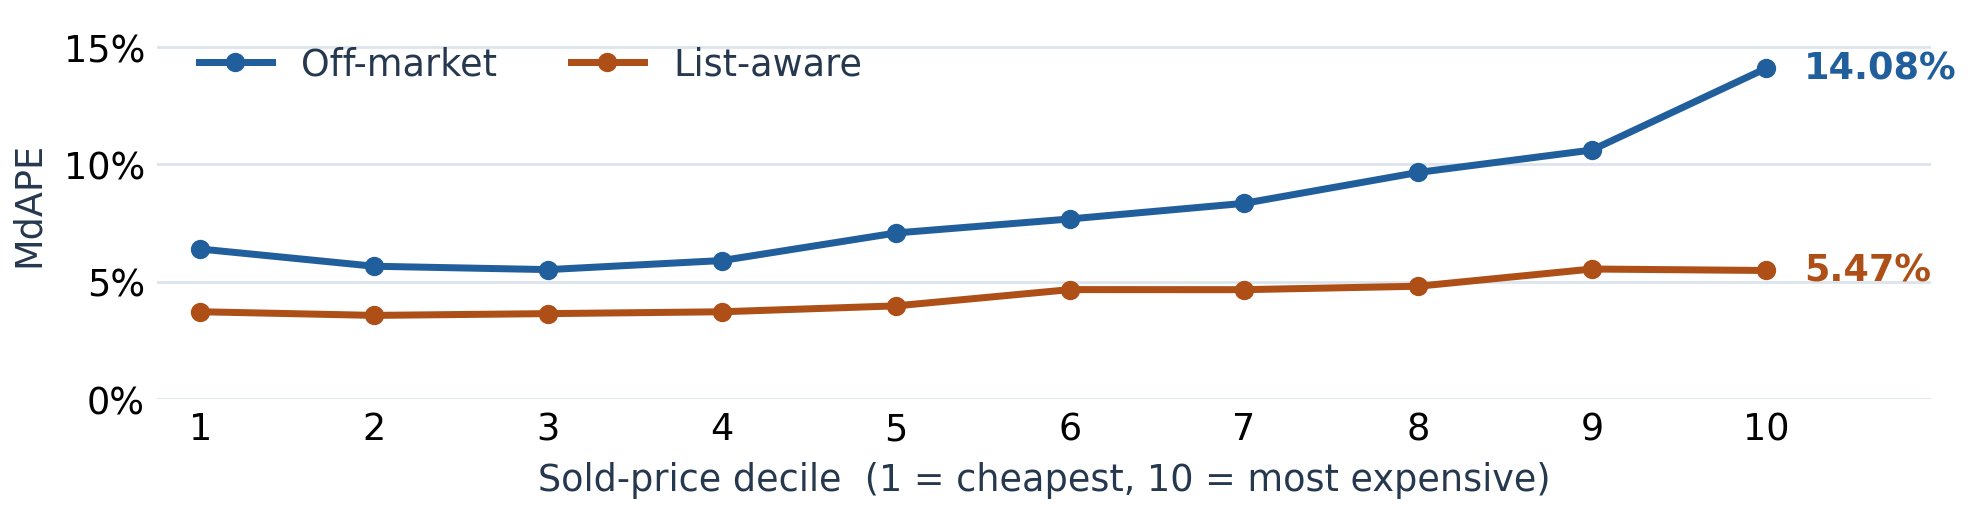
\includegraphics[width=.86\linewidth]{error_by_price_decile.png}
\end{center}
\vspace{-6pt}
Off-market MdAPE reached 14.08\% above \$1.76 million (top decile), with median signed error of $-8.56\%$. The cheapest decile had 6.39\% MdAPE and $+5.09\%$ signed error, consistent with predictions compressing price extremes. Top-decile MdAPE exceeded deciles 2--9 in all 36 communities with at least eight top-decile and twenty middle-decile sales. Across 90 neighborhoods with at least 50 sales, the 10th--90th percentile of neighborhood MdAPE was 6.06--9.71\%. Off-market MdAPE was 10.13\% for detached homes and 6.30\% for condo apartments. The list-aware top decile had 5.47\% MdAPE and near-zero median signed error.

\textbf{Limitations.} The 90th-percentile APE was 21.70\% off-market and 11.32\% list-aware. These are historical tails. The data use synthetic geography. About 64\% of validation listings predate their sale-month cutoff, so real listing-day use requires an as-of-listing evaluation.

\reportsection{Outside data and reproducibility}
The organizer dataset was our sole source. From the release root, use Python 3.12 and optionally set \texttt{DATA\_DIR} to the organizer's Parquet folder.
{\small
\begin{verbatim}
python -m pip install -r requirements.txt
export OMP_NUM_THREADS=4 OPENBLAS_NUM_THREADS=1
python run.py predict && python run.py check
python run.py validate && python run.py report
\end{verbatim}}
\end{document}
